\section{Proper (2,3)-poles}\label{ch:proper-23-poles}

To explore multipoles effectively, it is best to start with the simplest ones and gradually move towards more complex ones. That's why we begin by examining the $k$-poles starting from the smallest $k$. Specifically, the smallest $k$ for which it is interesting to explore the colourability of $k$-poles arising from snarks with $k$-edge-cuts is 4.
The~1-poles are trivially uncolourable.
For a 2-pole to be colourable, both of its semiedges must have the same colour.
Similarly, for a 3-pole, all three of its semiedges must have pairwise different colours. Also, the colouring properties of $4$-poles are already widely explored since their colouring properties are limited as well \cite{ChladnyFactorisation}.
The analysis of the colouring properties of $5$-pole comes from the following ideas of P. J. Cameron, A. G. Chetwynd and J. J. Watkins \cite{Cameron1987}.

%Another corollary of the Parity Lemma may be that for each 5-pole $M$ to be colourable, it needs to have three semiedges of one colour and the other two with a different colour each. The three semiedges coloured by the same colour in $\phi$ are called \textit{sociable} in $\phi$, and the other two coloured by a colour different from the others are called \textit{solitary} in $\phi$.
By the Parity Lemma, in each colouring $\phi$ of a $5$-pole $M$, three semiedges of $M$ have the same colour. We call these edges \textit{sociable} in $\phi$. The remaining two semiedges of $M$, called \emph{solitary} in $\phi$, are coloured by the remaining two colours.
Because the colouring set of $M$ is closed under a permutation of colours, it only matters which semiedges of $M$ may be solitary. Using this, we can visualize the colouring set of any 5-pole in the following way.
% Trochu iný návrh riadku vyššie:
%Since the colouring set of $M$ is closed under a permutaion of colours, we can decsribe $\text{col}(M)$ by specifying all pairs of semiedges of $M$ that are solitary in some colouring of $M$.

%Because of the isomorphism of colourings, it does not matter which colours we use in the colouring, but rather which semiedges are solitary. For a 5-pole $T(e_1,e_2,e_3,e_4,e_5)$ we denote by $R_T$ a graph with vertex set\linebreak $V=\{e_1,e_2,e_3,e_4,e_5\}$, in which for each $e_i,e_j\in V$, the graph contains an edge $e_ie_j$ if and only if there exists a colouring $\phi$ of $T$ such that the semiedges $e_i$ and $e_j$ are solitary in $\phi$. $R_T$ is called a \textit{colouring graph of T}. By \cref{lem:solitary}, $R_T$ has no pendant vertex \cite{Preissmann1983}.
For a 5-pole $M(e_1,e_2,e_3,e_4,e_5)$ we denote by $R_M$ a graph with the vertex set $V=\{e_1,e_2,e_3,e_4,e_5\}$, in which for each $e_i,e_j\in V$, the graph contains an edge $e_ie_j$ if and only if the semiedges $e_i$ and $e_j$ are solitary in some colouring of $M$. The graph $R_M$ is called the \textit{colouring graph of $M$}.
The colouring graph $R_M$ of any $5$-pole has no vertex of degree one \cite{Preissmann1983}.
% TODO: k tomuto sa možno dá dodať aj formulácia tej lemy alebo spomenúť ideu dôkazu

% Isomorfic colourings podľa mňa nepotrebujeme, nakoľko stačí hovoriť len o permutácii farieb.
%Let $M$ be a multipole, $\phi_1$ and $\phi_2$ colourings of $M$ such that $\phi_1$ uses $C=\{c_1,c_2,c_3\}$ as the set of colours and $\phi_2$ uses $D=\{d_1,d_2,d_3\}$. We say that $\phi_1$ and $\phi_2$ are \textit{isomorphic} if there exists a bijection $f\colon C\rightarrow D$ and for each edge $e$ from $E(M)$ $\phi_2(e)=f(\phi_1(e))$.
%
%Let $T$ be any proper (2,3)-pole. First, we can see that because of colouring isomorphism, if one colouring can be attained, then the colouring set of $T$ must contain this colouring along with all possible isomorphic colourings to the first one. Also, we can get a new colouring using the interchange of colours on a chain.
%
%\begin{lemma}[\cite{Preissmann1983}]
%	Let $T$ be a 5-pole and $\phi$ a colouring of $T$. Let $p$ and $q$ be its two solitary semiedges in $\phi$. Then there exists a sociable semiedge $p'$ and another colouring of $T$, in which $p'$ and $q$ are solitary.
%	\label{lem:solitary}
%\end{lemma}

From a case analysis in \cite{Preissmann1983}, it follows that if $M$ is a $5$-pole that can be completed to a snark by performing a junction with some colourable $5$-pole, then colouring graph $R_{M}$ of $M$ is a subgraph of:
\begin{itemize}
	\item a $5$-cycle, or
	\item the graph formed by two disjoint triangles sharing a single vertex, or
	\item the complement of $C_3$.
\end{itemize}
Accordingly, the $5$-pole $M$ whose colouring graphs are subgraphs of the mentioned graphs is called \textit{superpentagons}, \textit{negators} and \textit{proper $(2 ,3)$-poles}, respectively.

The colouring graph of a superpentagon is either empty or the $5$-cycle. The colouring graph of a negator is empty, consists of one triangle or consists of two edge-disjoint triangles with a common vertex.
%TODO: Zišlo by sa asi lepšie sformulovať.
Máčajová and Škoviera characterised which negators have which colouring graphs \cite{IrreducibleSnarksSkoviera}.
For proper $(2,3)$-poles, the situation is more diverse and their colouring graphs have not been studied yet.

%Using this theorem and the Parity lemma, it can be proven that if we get two colourable $5$-poles by severing five edges in a given snark, they can be only one of three types: negators, superpentagons and proper $(2,3)$-poles. For the first two, their colouring properties are already explored, which is why we chose to explore the last type.

A snark can be constructed from a proper (2,3)-pole by the junction of the semiedges in the connector of size two and joining the semiedges from the connector of size three to a new vertex. It can be proved, that since they are proper, the result is a snark. Conversely for each snark, the result after removing a vertex and severing an edge not incident with it will always be a proper (2,3)-pole.

By default, when we get a proper (2,3)-pole in this way, we denote it by $T(A,B)$, where the connector $A$ contains the two semiedges resulting from severing the edge and similarly, connector $B$ contains the three semiedges resulting from removing the vertex, such that $A=(a_1,a_2)$ and $B=(b_1,b_2,b_3)$. An example can be seen in \cref{fig:23-pole-example}.

\begin{figure*}
	\centering
	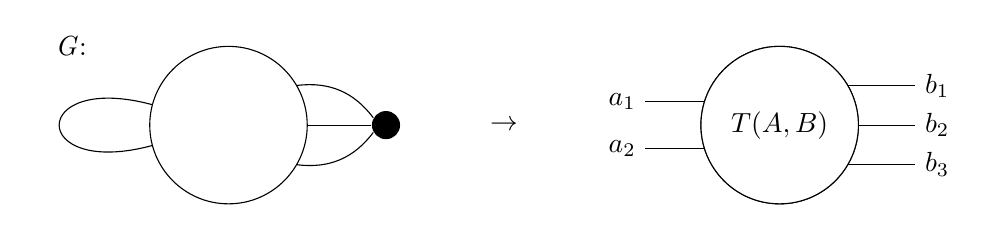
\begin{tikzpicture}[scale=1]
	\tikzset{every loop/.style={}}
	\node[draw=none] (G) at (-2, 1) {\textit{G}:};
	\node[shape=circle,draw=black, minimum size=2cm] (1) at (0,0) {};
	\node[shape=circle,color=black,fill,text width=1pt] (2) at (2,0) {};
	
	\path (1) edge (2);
	\path (1) edge [bend left] (2);
	\path (1) edge [bend right] (2);
	
	\path (1)
	edge (2)
	edge [loop left] node {} ()
	;
	
	\node[draw=none] (arrow) at (3.5, 0) {$\rightarrow$};

	\node[shape=circle,draw=black, minimum size=2cm] (1) at (7,0) {$T(A,B)$};
	\node[shape=rectangle,draw=none] (1mid) at (7,0) {$T(A,B)$};
	\node[draw=none] (2) at (9,0.5) {$b_1$};
	\node[draw=none] (3) at (9,0) {$b_2$};
	\node[draw=none] (4) at (9,-0.5) {$b_3$};
	
	\node[draw=none] (5) at (5,0.3) {$a_1$};
	\node[draw=none] (6) at (5,-0.3) {$a_2$};
	
	\draw (2) -- (2-|1mid.east);
	\draw (3) -- (3-|1mid.east);
	\draw (4) -- (4-|1mid.east);
	
	\draw (5) -- (5-|1mid.west);
	\draw (6) -- (6-|1mid.west);
	
	\node[shape=circle,draw=black,fill=white, minimum size=2cm] (1) at (7,0) {$T(A,B)$};
				
\end{tikzpicture}
	\caption{Creation of a proper $(2,3)$-pole from a snark $G$}
	\label{fig:23-pole-example}
\end{figure*}

By applying the knowledge about the multipoles being proper and the Parity lemma, it is clear that the colouring set of each proper (2,3)-pole is a subset of the set

$$\{(a_1,a_2,b_1,b_2,b_3)\in\mathbb{K}^5~|~a_1+a_2=b_1+b_2+b_3\neq 0\}.$$

We will refer to this set only as $C$ from now on. Note that in this definition, the~terms $a_1$ to $b_3$ denote the colours of the respective semiedges. The non-equality to zero is evident because they are proper, and the equality of flow through both connectors follows from the Parity lemma.

A proper (2,3)-pole is called \textit{perfect} if its colouring set coincides with the colouring set $C$.

%Another corollary of the Parity Lemma may be that for each 5-pole to be colourable, it needs to have three semiedges of one colour and the other two with a different colour each. This way, we can define so-called solitary and sociable semiedges.
%
%\begin{definition}
%	Let $M$ be a 5-pole and $\phi$ its colouring. The three semiedges coloured by the same colour are called \textit{sociable} in $\phi$, and the other two coloured by a colour different from the others are called \textit{solitary} in $\phi$.
%\end{definition}


%The idea behind the proof is that if $p$ has colour 1 and $q$ colour 2, we take into account a subgraph of $T$ formed by the edges with colours 1 and 3. In this partial graph, there is a path, which is called a (Kempe) chain, in which the extremities are $p$~and a~sociable semiedge $p'$. By the interchange of colours 1 and 3 along this chain, we obtain a new colouring of $T$ in which $p'$ and $q$ are solitary.

%Let $T$ be a 5-pole and $\phi$ its colouring. Then let $p$ and $q$ be its two solitary semiedges in this colouring, $2$ the colour of $p$ and $3$ the colour of $q$. In the partial graph $T'$ formed by the edges of colours $1$ and $2$ there is a chain which extremities are $p$ and a sociable semiedge $p_1$. By the interchange of colours $1$ and $2$ along this chain. we obtain a new colouring of $T$ in which $p_1$ and $q$ are solitary.



%Since the semiedges in proper (2,3)-poles are $(a_1,a_2,b_1,b_2,b_3)$, we can use them as the set of vertices in the colouring graphs of proper (2,3)-poles.

%\begin{figure}
%	\centering
%	\begin{tikzpicture}
	\graph[nodes={draw, circle, fill=black}, n=5, clockwise, radius=1.5cm]
{
	1/""[label={$a_1$}],
	2/""[label=right:$a_2$],
	3/""[label=below:$b_1$],
	4/""[label=below:$b_2$],
	 5/""[label=left:$b_3$]
};
\end{tikzpicture}
%	\caption{Vertices of a colouring graph of proper (2,3)-poles}
%	\label{fig:proper-associated-vertices}
%\end{figure}

%A 5-pole $T$ \textit{allows solitary cycle} $e_1e_2\cdots e_n$ if for each $i$ from 1 to $n-1$, $T$ allows a colouring, where $e_i$ and $e_{i+1}$ are solitary, including the colouring where $e_n$ and $e_1$ are solitary.
A 5-pole $T$ \textit{allows solitary cycle} $e_1e_2\cdots e_n$ if its colouring graph $R_T$ contains the cycle $e_1e_2\cdots e_n$.



\input chapters/23-colouring-classes.tex